\documentclass[12pt]{article}
\usepackage[utf8]{inputenc}
\usepackage{upquote}
\usepackage[margin=20mm]{geometry} 
\usepackage{amsmath,amsthm,amssymb}
\usepackage{graphicx}
\usepackage{listings}
\newenvironment{statement}[2][Statement]{\begin{trivlist}
\item[\hskip \labelsep {\bfseries #1}\hskip \labelsep {\bfseries #2.}]}{\end{trivlist}}
\usepackage{xcolor}

\usepackage{subfigure}


% Listings package for code rendering (No external dependencies)
\usepackage{listings}  
\usepackage{xcolor}   % Color support
\usepackage{tcolorbox} % Box for better appearance
\usepackage{enumitem} 
% Define custom colors for code highlighting
\definecolor{codegreen}{rgb}{0,0.6,0}
\definecolor{codegray}{rgb}{0.5,0.5,0.5}
\definecolor{codepurple}{rgb}{0.58,0,0.82}
\definecolor{backcolour}{rgb}{0.95,0.95,0.92}


\lstset{frame=tb,
    language=Python,
    backgroundcolor=\color{backcolour},   
    commentstyle=\color{codegreen},
    keywordstyle=\color{magenta},
    numberstyle=\tiny\color{codegray},
    stringstyle=\color{codepurple},
    basicstyle=\ttfamily\footnotesize,
    breakatwhitespace=false,         
    breaklines=true,                 
    keepspaces=true,                 
    numbers=left,       
    numbersep=5pt,                  
    showspaces=false,                
    showstringspaces=false,
    showtabs=false,                  
    tabsize=2,
}





\title{Assignment 3}


\begin{document}
\maketitle

\section{1 Complex numbers}
%wanjing

\subsection{} % 1.1

\textbf{(i)} 

\begin{equation}
\begin{aligned}
d &=(a_1 + i a_2) + (b_1 + i b_2) = (a_1 + b_1) + i\,(a_2 + b_2).
\end{aligned}
\end{equation}

\textbf{(ii)}
\begin{equation}
\begin{aligned}
d &=(a_1 + i a_2) - (b_1 + i b_2) = (a_1 - b_1) + i\,(a_2 - b_2).
\end{aligned}
\end{equation}

\textbf{(iii)} 
\begin{equation}
\begin{aligned}
d &=(a_1 + i a_2)(b_1 + i b_2) \\
&= a_1b_1 + i a_1b_2 + i a_2b_1 + i^2 a_2b_2\\
&= (a_1b_1 - a_2b_2) + i\,(a_1b_2 + a_2b_1).
\end{aligned}
\end{equation}

\textbf{(iv)} For the quotient 
\begin{equation}
\begin{aligned}
d &= \frac{a}{b} \\
&= \frac{a_1 + i\,a_2}{b_1 + i\,b_2}\\
&= \frac{(a_1 + i\,a_2)(b_1 - i\,b_2)}{(b_1 + i\,b_2)(b_1 - i\,b_2)}\\
&= \frac{(a_1 + i\,a_2)(b_1 - i\,b_2)}{b_1^2 + b_2^2} \\
&= \frac{a_1b_1 + a_2b_2 + i\,(a_2b_1 - a_1b_2)}{b_1^2 + b_2^2}\\
&= \frac{a_1b_1 + a_2b_2}{b_1^2+b_2^2} + i\,\frac{a_2b_1 - a_1b_2}{b_1^2+b_2^2}.
\end{aligned}
\end{equation}


\subsection{} % 1.2
by $\sqrt{-3} = \sqrt{3}\,i$ , we have $d = 0 + i\,\sqrt{3}$. 

\subsection{} % 1.3
\textbf{(i)} 
\begin{equation}
\begin{aligned}
d &= a \cdot b = a_r e^{i a_\theta} \cdot b_r e^{i b_\theta} = a_r b_r e^{i(a_\theta + b_\theta)}
\end{aligned}
\end{equation}


\textbf{(ii)} 

\begin{equation}
\begin{aligned}
d &=  \frac{a}{b} = \frac{a_r e^{i a_\theta}}{ b_r e^{i b_\theta}} =  \frac{a_r}{b_r} e^{i(a_\theta - b_\theta)}
\end{aligned}
\end{equation}

\subsection{} %1.4
\begin{equation}
\begin{aligned}
\overline{a_r e^{i a_\theta}} = a_r e^{-i a_\theta}.
\end{aligned}
\end{equation}

\subsection{}

Let 
\[
a = a_r e^{i a_\theta} = a_r (\cos a_\theta + i\sin a_\theta)
\]
and
\[
b = b_r e^{i b_\theta} = b_r (\cos b_\theta + i\sin b_\theta).
\]

\textbf{(i)}
\begin{equation}
\begin{aligned}
d &= a + b\\
& = \Bigl(a_r\cos a_\theta + b_r\cos b_\theta\Bigr) + i\Bigl(a_r\sin a_\theta + b_r\sin b_\theta\Bigr).
\end{aligned}
\end{equation}


\textbf{(ii)} For 
\begin{equation}
\begin{aligned}
d &= a + b\\
& = \Bigl(a_r\cos a_\theta - b_r\cos b_\theta\Bigr) + i\Bigl(a_r\sin a_\theta - b_r\sin b_\theta\Bigr).
\end{aligned}
\end{equation}
\subsection{}

The polar form is given by
\[
a = r\, e^{i\theta},
\]
where
\[
r = \sqrt{a_1^2 + a_2^2} \quad \text{and} \quad \theta = \arctan\!\left(\frac{a_2}{a_1}\right)
\]
So
\[
a = \sqrt{a_1^2+a_2^2}\; e^{i\arctan\!\left(\frac{a_2}{a_1}\right)}.
\]


\section{2 Fourier Transform – Theory}
%zhigao
\subsection{}
The Fourier Transform is:
\[F\{f\}(u) = F(u) = \int_{-\infty}^{\infty} f(x) \exp(-i 2\pi ux) \,dx\]
By using the Euler's formula(\(\exp(-i 2\pi ux) = \cos(2\pi ux) - i\sin(2\pi ux).\)), This formula can be rewritten as:
\[
F(u) = \int_{-\infty}^{\infty} f(x) \cos(2\pi ux) \,dx - i \int_{-\infty}^{\infty} f(x) \sin(2\pi ux) \,dx.
\]
\(\sin(2\pi ux)\) is an odd function that integrates to 0 on the symmetric interval.
\[
\int_{-\infty}^{\infty} f(x) \sin(2\pi ux) \,dx = 0.
\]
Hence, The imaginary part of \(F(u)\) is 0. \(F(u)\) is real.
\newline
Then, To verify that \(F(u)\) is an even function. I need to prove \(F(u) = F(-u)\).
Firstly, I got:
\[
F(-u) = \int_{-\infty}^{\infty} f(x) \exp(i 2\pi ux) \,dx.
\]
Then I can replace the variable \(-x\) to \(x'\), hence \(dx' = -dx\), so I got:
\[
F(-u) = \int_{\infty}^{-\infty} f(-x') \exp(-i 2\pi ux') (-dx') 
\]
From the question, the \(f\) is an even function, so \(f(-x')=f(x')\).
\(F(-u)\) can be rewritten as:

\[F(-u) = \int_{-\infty}^{\infty} f(x') \exp(-i 2\pi ux') \,dx' = F(u).\]
In summary, an even, real function is also even, real after Fourier transformed.
\subsection{}
\begin{enumerate}[label=(\roman*)]
  \item \[
\begin{aligned}
\int_{-\infty}^{\infty} b_a(x)\,dx 
&= \int_{-a/2}^{a/2} \frac{1}{a}\,dx  \\
&= \frac{1}{a} \times \Bigl(\tfrac{a}{2} - \bigl(-\tfrac{a}{2}\bigr)\Bigr) \\
&= \frac{1}{a} \times a \\
&= 1.
\end{aligned}
\]
Since the box function has values of \(\frac{1}{a}\) only on \([-\frac{a}{2},\frac{a}{2}]\), the upper and lower limits of the integral can be changed to \([-\frac{a}{2},\frac{a}{2}]\).
  \item
  By using the definition of the Fourier transform given in Bracewell Chapter 2:
  \[
    \int_{-\infty}^{\infty} f(x)\,\exp(-i2 \pi xs)\,dx.
    \]
  the box function could be written as:
    \[
B_a(k) 
= \int_{-\infty}^{\infty} b_a(x)\,\exp(-i2\pi kx)\,dx 
= \int_{-a/2}^{\,a/2} \frac{1}{a}\,\exp(-i2\pi kx)\,dx.
\]
Continue calculating:
\[
\begin{aligned}
B_a(k)
&= \frac{1}{a} \int_{-a/2}^{\,a/2} \exp(-i2\pi k x)\,dx \\[6pt]
&= \frac{1}{a} \,\biggl[\frac{\exp(-i2\pi kx)}{-i2\pi k}\biggr]_{x=-a/2}^{\,x=a/2}
&= \frac{1}{a} \cdot \frac{1}{-\,i\,2\pi\,k}
\bigl(\,\exp\bigl[-\,i\,2\pi\,k \cdot \tfrac{a}{2}\bigr]
 \;-\; \exp\bigl[-\,i\,2\pi\,k \cdot \bigl(-\tfrac{a}{2}\bigr)\bigr]\bigr).
\end{aligned}
\]
By the Euler's formula:
\[
e^{i\theta} = \cos(\theta) + i \sin(\theta), e^{-i\theta} = \cos(\theta) - i \sin(\theta)
\]
The function above could be rewritten as:
\[
B_a(k) 
= \frac{1}{a} \,\frac{-\,2\,i\,\sin\bigl(\pi\,a\,k\bigr)}{-\,i\,2\pi\,k}. = \frac{1}{\pi\,k\,a}\,\sin\bigl(\pi\,a\,k\bigr)
\]
Using the \(sinc(x) = \frac{sinx}{x}\), the final form of the Fourier transform of the box function is:
\[B_a(k) = sinc(\pi k a)\]

  \item 
  If \(a \rightarrow 0\), \(sin(ak\pi)\rightarrow 0\), and we know 
  \[
\lim_{z \to 0} \frac{\sin z}{z} = 1.
\]
 we can see \(ak\pi\) to \(z\), hence we get:
  \[
\lim_{a \to 0} \frac{\sin (ak\pi)}{ak\pi} = 1.
\]
  \item 
  I think if the box function is narrow in x space(a is near 0),  its Fourier transform will be wide in the k space(frequency domain). Conversely, if a is larger, then it is wider in x-space and narrower in k-space. This is the uncertainty property of the Fourier transform. this means a narrow function has a wide Fourier transform, and a wide function has a narrow Fourier transform.
\end{enumerate}
\section{3 Fourier Transform – In Practice}
%shuangcheng
\subsection{}
We use trui.png as the input image and apply Fourier Transform to calculate its spectrum. Figure \ref{fig:original} shows the input image. After calculating Fourier Transform, we get the power spectrum as shown in Figure \ref{fig:3.1}.

\begin{figure}[ht]
    \centering
    \subfigure[Original Figure trui.png]{
        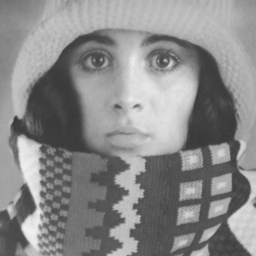
\includegraphics[width=0.4\columnwidth, keepaspectratio]{pics/trui.png}
        \label{fig:original}
    }
    \hfill
    \subfigure[Power Spectrum]{
        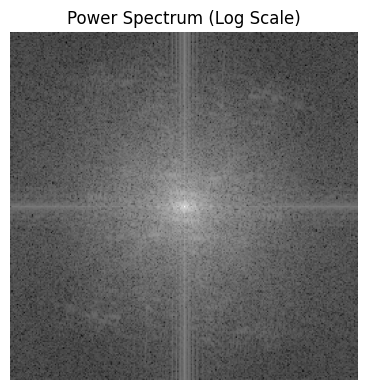
\includegraphics[width=0.4\columnwidth, keepaspectratio]{pics/a3-3.1.png}
        \label{fig:3.1}
    }
    \caption{Comparison of the Original Image and its Power Spectrum}
    \label{fig:comparison}
\end{figure}


By analyzing the power spectrum, we can observe that the low-frequency components are concentrated in the center, while the high-frequency components are distributed in the periphery.

We use the Python code shown in Listing 1 to calculate the Fourier transform.
\begin{lstlisting}[caption={Compute Power Spectrum Using 2D Fourier Transform},captionpos=b]
def compute_power_spectrum(image):
    fft_image = scipy.fft.fft2(image)  # Compute 2D FFT
    fft_shifted = scipy.fft.fftshift(fft_image)  # Shift zero frequency to center
    power_spectrum = np.log(1 + np.abs(fft_shifted))  # Log scale for better visualization
    return power_spectrum
\end{lstlisting}

Through Fourier transform, we can transform the image from the spatial domain to the frequency domain to analyze the frequency components of the image. This helps to identify noise, detect periodic structures, perform filtering, etc.

When calculating the Fourier transform, the default low-frequency part of the spectrum is located in the corner, so we use fftshift to move it to the center for a more intuitive analysis of the frequency components. In addition, the dynamic range of the spectrum value is large, and direct display will result in unclear high-frequency parts, so we use $\log(1 + |\text{FFT}|) $ for logarithmic transformation so that both low-frequency and high-frequency information can be well observed.

Through the power spectrum, we find that the image is mainly composed of low-frequency components, indicating that most of its areas are smoothly changing. In addition, in the high-frequency part, we can observe edge and detail information. Through Fourier transform, we can understand the frequency distribution of the image more clearly, which provides a basis for subsequent filtering operations. If the image contains more noise, the high-frequency part will be brighter. At this time, low-pass filtering can be used to remove the noise, but this may cause the image to become blurred.

\subsection{}
Figure \ref{fig:3.2} shows the input image and output results, where:

\begin{figure}[ht]
        \centering
      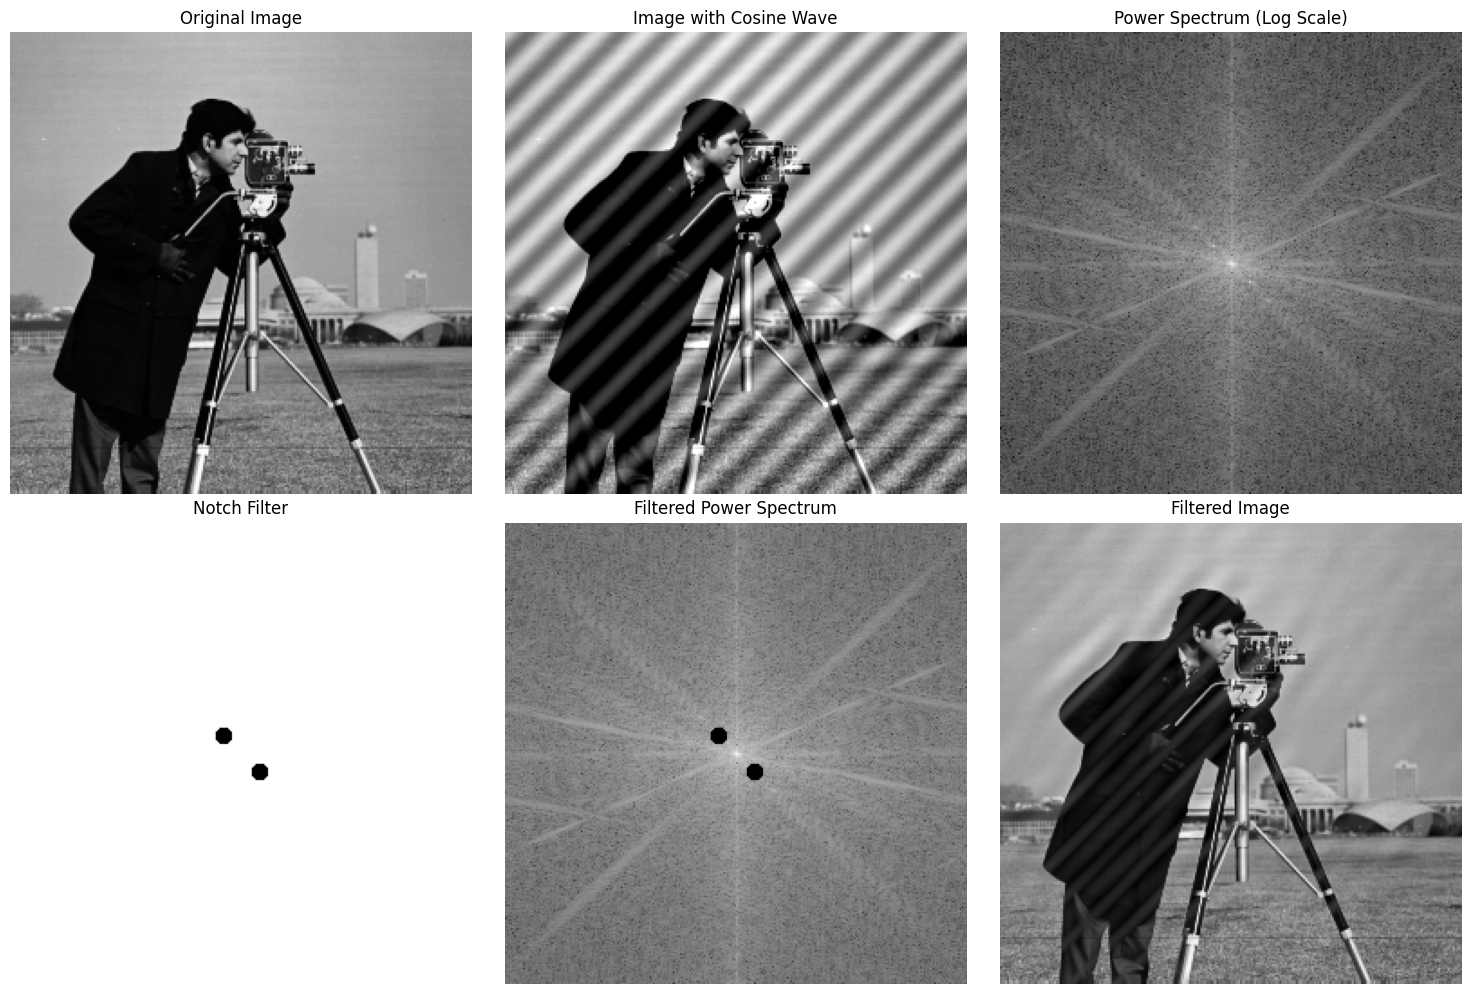
\includegraphics[width=1.0\columnwidth, keepaspectratio]{pics/a3-3.2.png}
        \caption[]{Input and Outputs}
    \label{fig:3.2}
    \end{figure}
The original input image is cameraman.tif, which is a standard grayscale image with clear edges and textures.

Image with Cosine Wave: A cosine interference wave is added to the original image to simulate periodic noise.

Power Spectrum (Log Scale): The spectrum of the image is calculated and visualized through Fourier transform.

Notch Filter: A notch filter is designed to remove interference waves of specific frequencies.

Filtered Power Spectrum: Shows the changes in the spectrum after filtering.

Filtered image: The final image after notch filtering.

We use the Python code shown as follow to finish the problem.
\begin{lstlisting}[caption={crucial Python Code Snippet},captionpos=b]
# Generate cosine wave interference
def add_cosine_wave(image, a0=50, v0=10, w0=10):
    H, W = image.shape
    x = np.arange(W)
    y = np.arange(H)
    X, Y = np.meshgrid(x, y)

    wave = a0 * np.cos(2 * np.pi * (v0 * X / W + w0 * Y / H))  # Normalize frequency
    noisy_image = np.clip(image + wave, 0, 255)  # Ensure pixel values remain in [0, 255]
    return noisy_image.astype(np.uint8)

noisy_image = add_cosine_wave(image)
F_noisy = fft2(noisy_image)
F_noisy_shifted = fftshift(F_noisy)
power_spectrum = np.log(1 + np.abs(F_noisy_shifted))

# Design a notch filter to remove interference
def notch_filter(shape, v0, w0, radius=5):
    H, W = shape
    X, Y = np.meshgrid(np.arange(W), np.arange(H))
    X = X - W // 2
    Y = Y - H // 2
    D1 = np.sqrt((X - v0) ** 2 + (Y - w0) ** 2)
    D2 = np.sqrt((X + v0) ** 2 + (Y + w0) ** 2)
    H = np.ones((H, W))
    H[D1 < radius] = 0  # Suppress frequency at (v0, w0)
    H[D2 < radius] = 0  # Suppress frequency at (-v0, -w0)
    return H

notch = notch_filter(image.shape, v0=10, w0=10)
F_filtered = F_noisy_shifted * notch
filtered_image = np.abs(ifft2(fftshift(F_filtered)))
\end{lstlisting}
In this experiment, we explored how to remove periodic stripe noise in the frequency domain and evaluated the effectiveness of Notch filtering. Using the Fourier transform, we converted the image from the spatial domain to the frequency domain, allowing us to observe and analyze its frequency components. For images affected by periodic interference, these disturbances typically manifest as distinct bright spots in the frequency domain. Therefore, we can identify the noise’s frequency distribution through spectrum analysis and design appropriate filters to eliminate it.

During processing, we first introduced a cosine wave interference into the original image, creating a regular stripe pattern in the spatial domain. We then computed its power spectrum and applied fftshift to center the low-frequency components, making the spectral distribution more intuitive to analyze. After examining the power spectrum, we observed that the interference stripes corresponded to two symmetrical bright spots. Based on this information, we manually selected the relevant frequency positions and designed a Notch filter to suppress these specific frequency components. Finally, we applied an inverse Fourier transform to the filtered spectrum to reconstruct the processed image.

The experimental results demonstrate that the Notch filter effectively removes periodic interference and significantly reduces stripe noise. However, since the filter selection influences surrounding frequency components, some image details may be lost. Additionally, the filter parameters require manual adjustment and cannot automatically adapt to different types of noise. In practical applications, adaptive frequency detection methods can be incorporated to automatically identify interference frequencies and optimize filter design, thereby enhancing the robustness and applicability of the denoising process.

\subsection{}

\begin{lstlisting}[caption={Compute Spatial Derivatives},captionpos=b]
def frequency_derivative(image, order_x=1, order_y=1):
    image = image.astype(np.float32)  # Convert image to float for numerical stability

    # Get image dimensions
    h, w = image.shape

    # Generate frequency domain coordinates
    u = np.fft.fftfreq(w) * w
    v = np.fft.fftfreq(h) * h
    U, V = np.meshgrid(u, v, indexing="xy")

    U[U == 0] = 1e-6
    V[V == 0] = 1e-6

    D_x = (1j * 2 * np.pi * U) * (order_x > 0)
    D_y = (1j * 2 * np.pi * V) * (order_y > 0)
    D = fftshift(D_x + D_y)

    F_image = fftshift(fft2(image))
    F_derivative = F_image * D
    derivative_image = np.real(ifft2(ifftshift(F_derivative)))

    # Normalize the output for visualization
    derivative_image = np.abs(derivative_image)
    derivative_image = derivative_image / np.max(derivative_image) * 255

    return derivative_image.astype(np.uint8)


# Calculate derivatives in different directions
derivative_x1_y0 = frequency_derivative(image, order_x=1, order_y=0)  # x
'''
The calculations for other directions are basically the same as above and will not be repeated here.
'''
\end{lstlisting}

Figure \ref{fig:3.3} shows the illustrations of the function applied to cameraman.tif at different combinations of orders of derivatives.

\begin{figure}[ht]
        \centering
      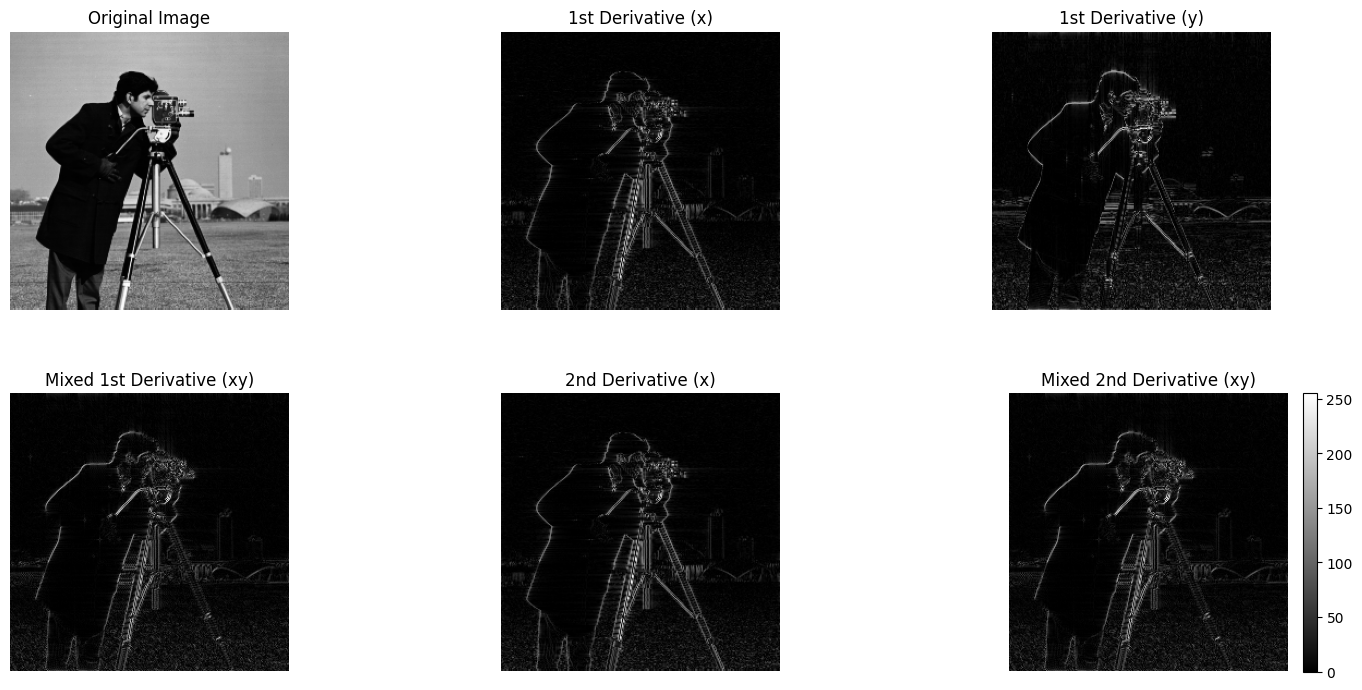
\includegraphics[width=1.0\columnwidth, keepaspectratio]{pics/a3-3.3.png}
        \caption[]{Input and Outputs}
    \label{fig:3.3}
    \end{figure}

Spatial derivatives can be efficiently computed in the frequency domain by multiplying an image’s Fourier Transform with a derivative kernel. Using the convolution theorem, we implemented a function that takes two derivative orders (one for the x-direction and one for the y-direction) and returns the corresponding partial derivative of a given image.

The function first converts the image to the frequency domain using the Fourier Transform. It then applies a derivative filter by multiplying the transformed image with frequency domain operators. To ensure numerical stability, zero-frequency components were adjusted to prevent division errors. Finally, the inverse Fourier Transform is applied to obtain the spatial derivative.

We tested the function on a grayscale image, computing first- and second-order derivatives in different directions. The resulting images highlight edges and fine details associated with each derivative order. A colorbar is included to aid visualization. Below, we present the function implementation along with the corresponding results.

\end{document}
